%%%%%%%%%%%%%%%%%%%%%%%%%%%%%%%%%%%%%%%%%%%%%%%%%%%%%%%%%%%%%%%%%%%%%%%%%%

%%%%%                           Conclusion Géné                     %%%%%%
%%%%%%%%%%%%%%%%%%%%%%%%%%%%%%%%%%%%%%%%%%%%%%%%%%%%%%%%%%%%%%%%%%%%%%%%%%

\phantomsection 
\addcontentsline{toc}{chapter}{General conclusion} \mtcaddchapter
\addtocontents{toc}{\protect\addvspace{10pt}}

\vspace*{-1cm}
\begin{flushright}
\section*{\fontsize{20pt}{20pt}\selectfont\textnormal{General conclusion}}
\end{flushright}
\vspace{2cm}

\lhead[\fancyplain{}{General conclusion}]
      {\fancyplain{}{}}
\chead[\fancyplain{}{}]
      {\fancyplain{}{}}
\rhead[\fancyplain{}{}] 
      {\fancyplain{}{General conclusion}}
\lfoot[\fancyplain{}{}]
      {\fancyplain{}{}}
\cfoot[\fancyplain{}{\thepage}]
      {\fancyplain{}{\thepage}}
\rfoot[\fancyplain{}{}]
     {\fancyplain{}{\scriptsize}}

%%%%%%%%%%%%%%%%%%%%%%%%%%%%%%%%%%%%%%%%%%%%%%%%%%%%%%%%%%%%%%%%%%%%%%%%%%
%%%%%                      Start part here                          %%%%%%
%%%%%%%%%%%%%%%%%%%%%%%%%%%%%%%%%%%%%%%%%%%%%%%%%%%%%%%%%%%%%%%%%%%%%%%%%%

\section*{Outcomes}

Aside from the athletes themselves (their natural skills, life circumstances, and personal drive), coaching expertise is one of the most significant parameters in sports performance enhancement. This expertise comes both from subjective intuition and experience, and from the various scientific resources to which the coaches have access. 

However, the constraints of science often make the research setting and parameters very different from the reality in the field. 
Research reduces problems to only a few variables for the sake of rigor, while coaching is more holistic and practical, though not always evidence-based. 
% In order to be able to conduct rigorous research, the human body and its motion must be simplified. On the other hand, in order to keep being relevant to the reality of training, coaching methods cannot be fully rigorous. All this means that there is a trade-off between the complexity of research methods and the complexity of the human body in movement. Consequently, research outcomes may not be applicable to the coach's daily practice, but coaching practices are . 
Research is a long-term and complicated process, while coaches need quasi real-time feedback which is easily accessible. 
Some research findings can be lost in the translation to layman's terms, while on the other hand, research may employ very convoluted methods to "state the obvious," or focus on areas that are not relevant. 
Consequently, there is a need to for better understanding of both research and coaching needs and constraints, in order to make the first more applicable and less reductive, and to mitigate the application of unfounded beliefs in the second.

% Experience-based coaching intuition will always be of paramount importance, but 
New research tools can shed unbiased light on movement analysis and offer new perspectives to coaches. In this regard, recent advances in markerless kinematics offer a promising perspective. Until recently, sports motion analysis had to be performed either with intrusive and complex marker-based techniques, or with rough and inaccurate markerless options. Thankfully, the last few years have been prolific in the development of markerless technology. It is now possible to go without markers and still obtain coherent, although imperfect, 3D full-body joint kinematics. These methods are usually more robust than marker-based ones, and they are rapidly becoming more and more accurate. 

Our decision to craft a robust triangulation procedure, and to constrain rough 3D coordinates to a biomechanically consistent skeletal model, makes results almost as accurate as marker-based ones, at least for walking, running, ergometer cycling, and boxing. Such an approach has also been proven to work in the field, under constraints which would make it difficult to set up a whole research-grade system. It is also possible to use lightweight, wireless, consumer-grade cameras, despite they are not straightforward to calibrate and synchronize. Sports equipment can be detected along with the athlete, with the caveat that, much like with marker-based techniques, inverse kinematics is still an open challenge when closed-loop constraints are enforced. Both in boxing and in BMX racing, key performance indicators are satisfactorily retrieved. 

The Pose2Sim workflow we proposed uses 
% aimed at building a bridge between the computer vision and biomechanics communities, by using 
two renowned tools of their respective fields: OpenPose for 2D pose estimation, and OpenSim for 3D joint kinematics. This workflow is open-source, versatile, and accessible for sports scientists who are the target audience, rather than computer vision specialists. Pose2Sim was made to be useful and usable, and hence it is also being used: the University of Bath is creating a GUI around it, a (non-free) Blender add-on integrating it has been released \cite{Barreto2022}, and our GitHub repository is active. Pose2Sim has also been quoted by the University of Stanford, which later developed their own 3D markerless solution \cite{Uhlrich2022}. 

% \vskip 0.4cm


\section*{Limits and Perspectives}

Some challenges remain, which could determine the adoption of markerless kinematic tools by the community of sports sciences. According to many of the issues reported on the GitHub repository, the main stumbling block for users is calibration. Hence, there is a definite need for an easier procedure, such as the one proposed by \cite{Argus}. It would even be worth testing an auto-calibration method, based on the knowledge of the size of a limb, tracked across multiple views. As we have demonstrated, an imperfect calibration does not degrade results much once 3D reconstruction has been constrained to a skeletal model. 

Moreover, the feedback given to athletes and coaches should be provided quickly enough for them to integrate it, so that they can adjust their motion patterns before their next trial sequence. Quasi-real-time can be achieved with research-grade cameras, as videos are directly downloaded after each sequence on the master computer, which can run Pose2Sim in the background. For wireless consumer-grade cameras, it is more complicated, although downloading media can sometimes be done remotely, without risking impairment of the camera calibration. 

Additionally, by their nature, team sports are practiced in groups, and thus performing multi-person inverse kinematics can be important. Although we have not yet implemented it, we have described possible methods to achieve such a task. \cite{Easymocap2021} deals with this problem, and its approach could be integrated as a submodule in Pose2Sim. Another open issue is the implementation of constraints in case of multiple closed kinematic loops such as in cycling. Solving this could give more accurate results even when large occlusions occur.

Finally, sports scientists are usually more at ease with graphical user interfaces than with command line, and coaches prefer intuitive visual feedback rather than charts of joint angle waveforms. A visualization tool for Maya has been developed, but it is not yet ready for release. As all the tools used and proposed here are open-source, it would make more sense to propose it as a free standalone software application, or as a Blender add-on. See Figure~\ref{fig_blendermocap} for planned features, and Figure~\ref{fig_mayamocap} for those already developed on the Maya-MoCap toolbox. The work presented in this thesis has given rise to a projected collaboration with the University of Bath, which is currently developing a GUI for Pose2Sim, and with whom we plan to build a new sports dataset for more accurate markerless kinematics. 

% \vskip 0.4cm

\section*{Future Prospects}
Current datasets for 2D pose estimation are not accurately labelled, they suffer from a dearth of keypoints, and they are not trained to recognize either sports poses or to detect sports equipment. Building a whole new dataset could solve these issues. The dataset should be large and diverse, represent a wide variety of body types and of sports movements \cite{Seethapathi2019}, and include images with motion blur such as found in sports videos. The images in this dataset should not include any markers, since these could be interpreted as visual cues, which are not available in real sports situations. Finally, they should be labelled accurately. One way to do this is to build a synthetic dataset. 

For example, a mass of .c3d motion files could be gathered from various sports and be used to fit an SMPL+H mesh \cite{Pavlakos2019}, for example with the AMASS algorithm \cite{Mahmood2019}. These data could be augmented with already existing datasets for daily life activities, such as Agora \cite{Patel2021}. Multiple persons should be present in the scene, and they should occasionally be using sports equipment. Then, random clothing, background, and light could be added (see \cite{Wood2021,Bolanos2021} for a detailed workflow). Body types could also be modified simply by altering SMPL shape parameters. Numerous virtual cameras could then be placed in the scene, in order to gather a large and diverse number of perspective points.

Labelling human beings could theoretically be done on one single SMPL mesh, since the SMPL topology is constant. Consequently, one could assume that the positions of the annotated keypoints on the mesh would be consistently propagated to other frames, other poses, and other body shapes. This labelling technique could be termed "virtual palpation". As many virtual markers as needed could be used, for a precise evaluation of any movement and pose. However, only an expert should perform this task, and make sure that markers are correctly positioned: crowd-sourcing this task, as is done for more basic image classification and segmentation such as with ImageNet \cite{Deng2009}, has been proved to lead to systematic offset errors \cite{Needham2021b}. Finally, 3D virtual markers could be automatically projected on the 2D camera planes. This would result in an extensive sports dataset, created with minimal labelling work, on a potentially infinite number of views. 

Nevertheless, before training the network, one should make sure that the generated data are as diverse as the real world, by using one of the metrics proposed by \cite{Borji2019, Borji2022}. Additionally, keypoint positions need to be precise enough: SMPL shape vertices can sometimes be more than 5 cm apart, which could cause imprecision errors similar to soft tissue artifacts. 

\vspace*{1.5cm}
More generally, it would be useful to obtain precise joint kinematics with fewer cameras. On the one hand, thanks to the use of a constrained biomechanical model, coherent full-body 3D kinematics can be obtained from inaccurate coordinates of very few keypoints. On the other hand, with the proposed procedure, some information is lost at every stage of the workflow. Only a few keypoints are used to characterize a complex scene, the detection of these keypoints is reduced to their maximum likelihood instead of taking advantage of the whole heatmap, and when equipment is used, closed-loop constraints are not used for constraining the kinematic analysis yet. 

Further information could be inferred by detecting not only keypoints, but also shape, which would arguably provide additional visual clues. The dataset described above could allow this. Moreover, information could be extracted not only from space, but also from time. Hence, inverse kinematics using Kalman filters is a potential area of interest, especially since they can be used evaluate not only joint angles, but also velocities, accelerations, forces, and other kinetic variables. However, more research is needed to address singularity issues of Kalman filters and to provide working standards for the initialization of covariances.

Finally, deep-learning based kinematics is still at its infancy, and many perspectives are still to be explored. Some models could directly be trained to estimate joint angles from calibrated videos, without the need for 2D pose estimation, triangulation, and inverse kinematic steps, which are all the causes of some loss of data. In particular, physics-informed neural networks should be prospected.



\vspace*{\fill}
\begin{flushright}
\textit{"Research is to see what everybody has seen, and think what nobody has thought."} \\
Albert Szent-Gyorgyi
\end{flushright}


\begin{figure}[hbtp]
      \centering
      \Rotatebox{90}{
      \def\svgwidth{1\columnwidth}
      \fontsize{10pt}{10pt}\selectfont
      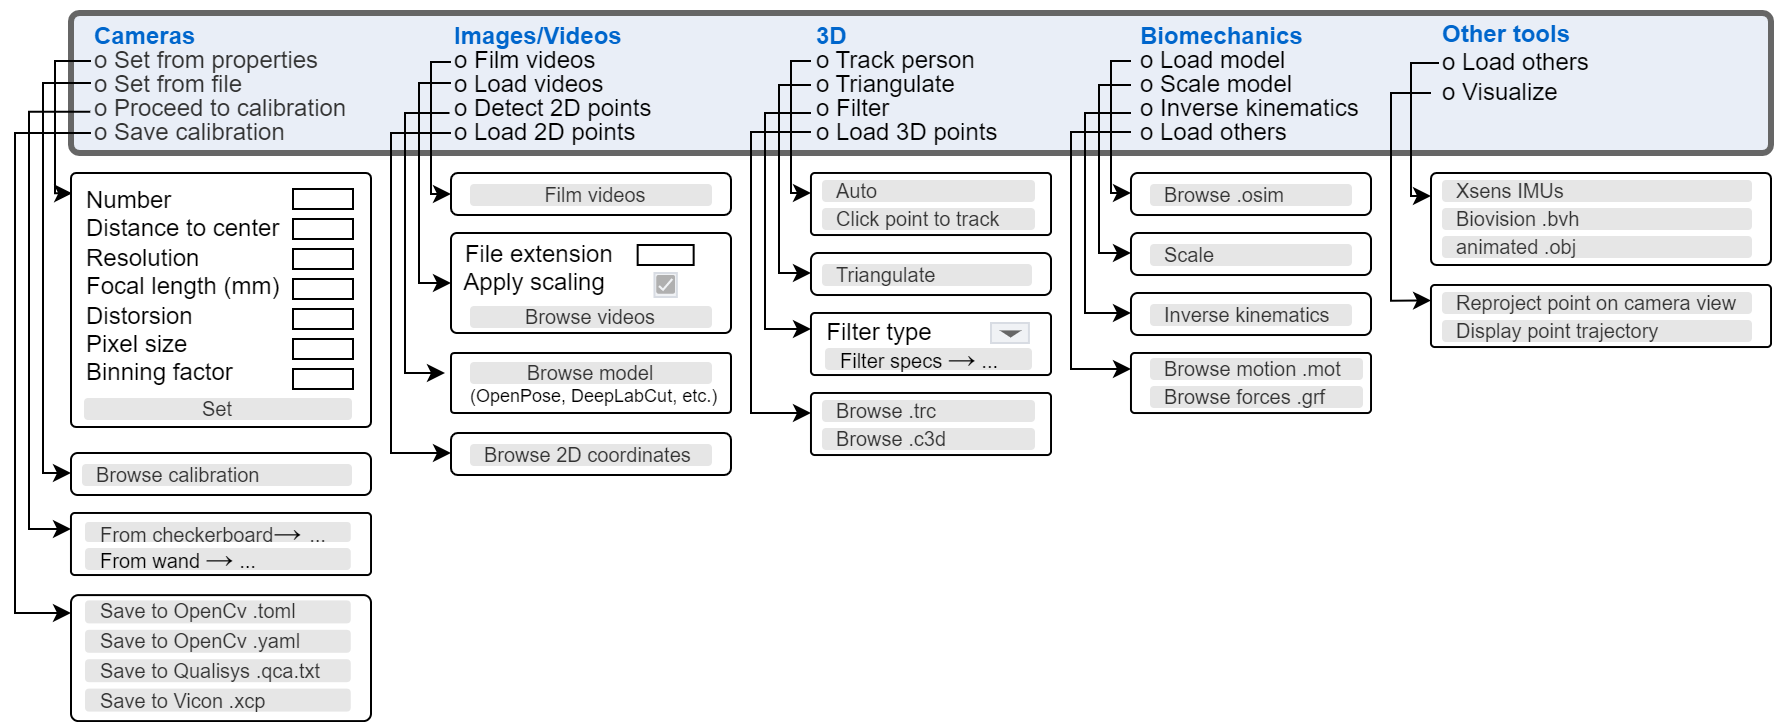
\includegraphics[height=0.6\linewidth]{"../Chap3/Figures/Fig_MayaMocap3.png"}}
      \caption{Planned features of the future Blender add-on. See Figure~\ref{fig_mayamocap} for reference to the already developed Maya-Mocap add-on.}
      \label{fig_blendermocap}
\end{figure}




% marche course vélo bmx boxe chill nage danse (lancer, parkour?)